\documentclass{article}
\usepackage[utf8]{inputenc}
\usepackage{geometry}
\usepackage{pgfplots}
\usepackage{graphicx}
\usepackage{verbatim}
\usepackage{amssymb}
\usepackage{amsmath}
\usepackage{tcolorbox} %needed
\usepackage{physics}
\usepackage{multicol}
\usepackage{hyperref}
\tcbuselibrary{listingsutf8}
\newcommand{\cls}{^{\circ}}


\geometry{a4paper, left=2cm, right=2cm, top=1cm, bottom=2cm}
\pgfplotsset{compat=1.18}

\begin{document}
I. Dibuja un ciclo de Carnot en un diagrama TS. Explica tu respuesta. \\
\textit{He realizado este diagrama en geogebra, el enlace interactivo se encuentra en el siguiente link:} \\ \href{https://www.geogebra.org/calculator/wtmndqjx}{https://www.geogebra.org/calculator/wtmndqjx}. \textit{Ignórese las letras minúsculas a un lado de cada flecha, he usado la herramienta vector para indicar la dirección del ciclo pero no es posible desaparecerlas; la explicación a grandes rasgos es que en el proceso de $ A \rightarrow B$ ocurre una expansión (incrementa el volumen) pero esta se encuentra en la misma franja de temperatura, a pesar de estar curveada en el diagrama P vs V este corresponde en este segmento a una isoterma por lo que en el eje T se verá como una constante que avanza sobre la entropía, la entropía "avanza" porque existe una varianza en el calor transferido y la temperatura de forma reversible. En el segmento $B \rightarrow C$ sigue aumentando el volumen pero con distinta temperatura, esta es la expansión adiabática que por sus condiciones detiene la transferencia de calor (sí, transferencia, pues de ser un refrigerador de carnot cambia el sentido de algunas cosas), esta expansión enfría al gas sin poder absorber calor para mantener su temperatura constante, como no existe transferencia de calor en este segmento entonces la entropía se mantiene constante por lo que al solo cambiar de temperatura para enfriarse por adquirir mayor volumen se verá como una línea vertical, en $C \rightarrow D$ es muy similar que $A \rightarrow B$ solo que este segmento isotérmico disminuye el volumen por lo que es una compresión isoterma, el calor y por tanto la entropía "corren en el sentido contrario" a como lo habían hecho antes por lo que ahora esto se verá como la temperatura fría constante mientras corre negativamente por el eje de la entropía, finalmente en el segmento $D \rightarrow A$ el volumen otra vez disminuye y la temperatura no pertenece a la misma franja pues esta regresa a ser la temperatura caliente por lo que análogo pero contrario a $ B \rightarrow C$ ocurre una compresión adiabática en el que se observará ilustrado como una línea vertical que mantiene la entropía (por el mismo argumento de la no transferencia de calor antes dada) pero la temperatura corre desde la temperatura fría hacia la caliente por lo que sube.} \\
\begin{figure} [h]
    \centering
    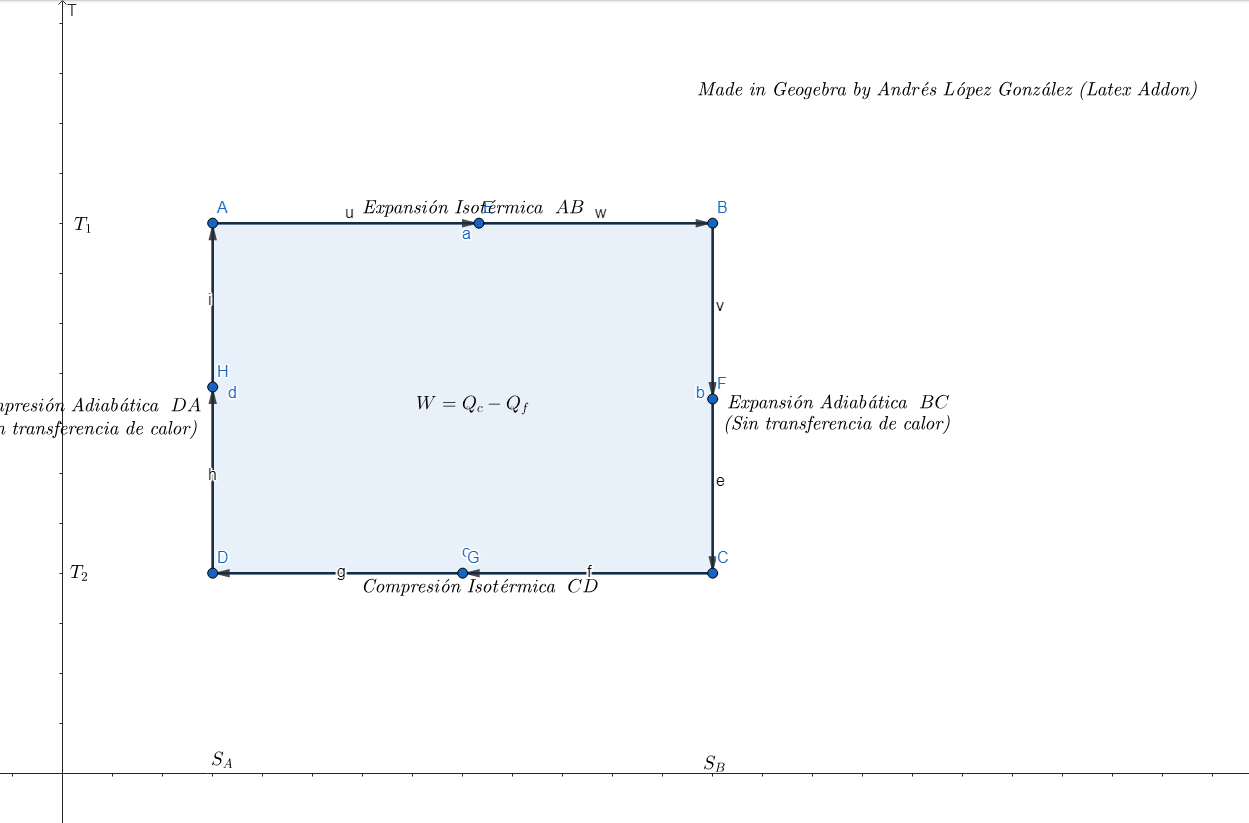
\includegraphics[width=0.8\linewidth]{Diagrama T vs S.png}
    \caption{Temperature vs Entropy; Carnot Cycle Diagram.}
    \label{fig:enter-label}
\end{figure} \\
II. ¿Puede una bomba de calor tener un coeficiente de rendimiento menor a 1? Explica tu respuesta. \\
\textit{Brevemente, sí. El coeficiente de rendimiento COP se define como la relación entre la cantidad de calor transferida desde un ambiente más frío hacia uno más caliente y la cantidad de trabajo que se debe realizar para lograr esta transferencia de calor. Esto se expresa como $COP = \frac{Q_c}{W}$, donde por convención $Q_c$ es la cantidad de calor transferida desde el ambiente frío y W es el trabajo realizado.} \\

\textit{Si el COP es menor a 1, significa que la cantidad de calor transferida desde el ambiente frío es menor que la cantidad de trabajo realizado. Esto es posible porque la bomba de calor no solo transfiere calor del ambiente frío al caliente, sino que también requiere trabajo para hacerlo.} 
\newpage
III. En un proceso termodinámico el cambio de entropía es de -80 J/K. ¿Qué puedes concluir del cambio de entropía en los alrededores? \\
\textit{Un cambio de entropía negativo como el que se describe (-80 J/K) en los alrededores indica una disminución en la dispersión de la energía en el entorno (caos del sistema), de forma más informal pero aterrizada, los valores entre Q y W en el sistema varían. La segunda ley de la termodinámica establece que la entropía de un sistema aislado tiende a aumentar con el tiempo, por lo tanto, un cambio negativo sugiere que además de evidentemente el proceso que está ocurriendo en el sistema en cuestión es no espontáneo, el sistema "transfiere" entropía al entorno, decreciendo así su entropía a costa de elevar la de su entorno, i.e. el "orden" de sí mismo a costa de aumentar el caos en sus alrededores. Separar en casos haría este inciso eterno por ello he usado implicaciones de la segunda ley de la termodinámica, pero es interesante ver que en el caso de la entropía por su definición integral de un ciclo reversible obtenemos de la siguiente ecuación donde delta hace referencia al diferencial que los "diferenciales de Q" debido a la orientación/sentido de su trayectoria nos otorgan valores negativos de la entropía}  \\
\begin{equation}
    \oint \delta S = \oint \frac{\delta Q}{T} < 0
\end{equation}
IV. Si una máquina térmica trabaja entre 100K y 500K, absorbe en cada ciclo 1000J de energía en forma de calor del reservorio a mayor temperatura, y tiene una eficiencia de 20\%, ¿puedes determinar si la máquina funciona de manera reversible o irreversible? \\
\textit{Para determinar si la máquina térmica funciona de manera reversible o irreversible, podemos utilizar el concepto de eficiencia de Carnot y compararlo con la eficiencia de la máquina dada. La eficiencia de Carnot por lo demostrado en clase se puede expresar con el cociente entre temperaturas sustituido por el cociente entre calores.
\begin{equation}
    e_{carnot} = 1 - \frac{T_f}{T_c}
\end{equation}
Sustituyendo...
\begin{equation*}
    e_{carnot} = 1 - \frac{100 \cls K}{500 \cls K} = 0.8 = 80\%
\end{equation*}
Por el enunciado la eficiencia de la máquina retornada es del 20\%, i.e. $e_{real} = 20\%$. Por otro lado al saber que la máquina trabaja entre temperaturas de 100K y 500K deducimos que el máximo posible de eficiencia para esta diferencia de temperatura es del 80\%; obsérvese que la máquina funciona de manera irreversible, pues su eficiencia registrada es significativamente menor a la eficiencia máxima de Carnot para las mismas temperaturas de trabajo. En los procesos reversibles la eficiencia de Carnot proporciona el límite máximo de eficiencia que puede alcanzarse.} \\
V. Un refrigerador de Carnot funciona con 18 moles de un gas ideal monoatómico, trabaja entre las
temperaturas de 450K y 150K y se realiza sobre él un trabajo de 120 Joules. \\
a) Dibuja el ciclo en un diagrama PV y calcula el coeficiente de rendimiento (COP) \\
\textit{Adjunto enlace de mi diagrama realizado en geogebra en el siguiente enlace \href{https://www.geogebra.org/calculator/dv9qrfyv}{https://www.geogebra.org/calculator/dv9qrfyv}, considérese que el sentido del diagrama va en sentido alfabético por lo que comienza con una expansión adiabática.}
\begin{figure} [h]
    \centering
    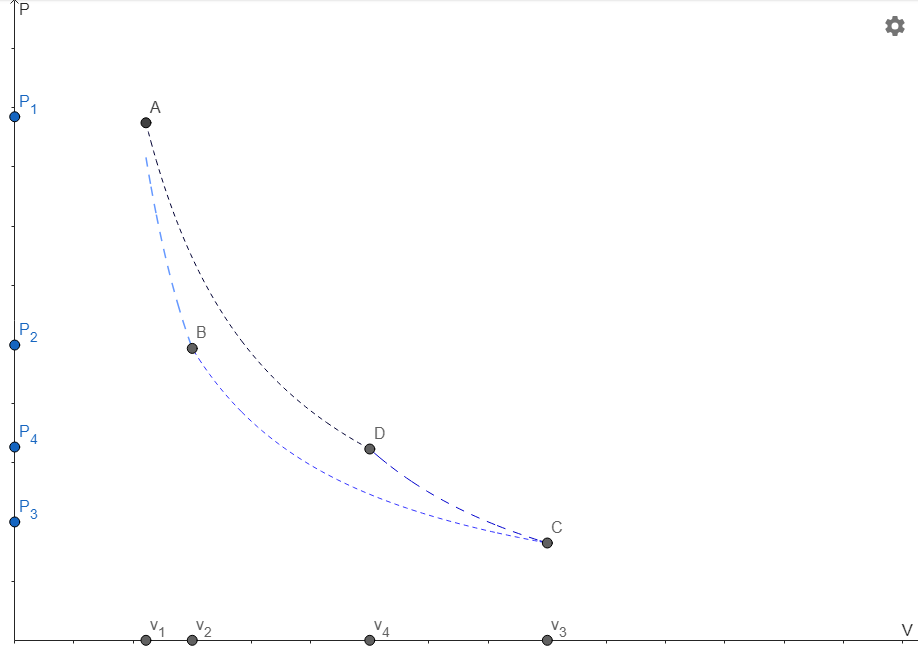
\includegraphics[width=0.6\linewidth]{V.png}
    \caption{Diagrama P vs V de Refrigerador de Carnot.}
    \label{fig:enter-label}
\end{figure} \\
\textit{Se sigue de la ecuación para el coeficiente de rendimiento (COP) en un refrigerador de Carnot}
\begin{equation}
    COP = \frac{1}{\frac{T_c}{T_f}-1}
\end{equation}
b) Sabiendo que después de la expansión isotérmica el volumen del gas es de $0.5m^3$ , calcula la presión y el volumen después de la compresión adiabática. \\
\textit{Obtenemos la eficiencia de carnot utilizando la ecuación que lo relaciona con el cociente entre temperaturas, para posteriormente igualarla con la relación del calor rechazado y el trabajo ejercido.}
\begin{equation}
    e = 1 - \frac{T_f}{T_c} = \frac{Q_r}{W} \quad \Rightarrow \quad Q_r = W \cdot \left[ 1 - \frac{T_f}{T_c} \right]
\end{equation}
\textit{Sustituyendo...}
\begin{equation*}
    Q_r = 120J \cdot \left[ 1 - \frac{150 \cls K}{450 \cls L} \right] =  \frac{120J \cdot 2}{3} = 80J
\end{equation*}
\textit{Nótese que el calor rechazado durante la compresión isotérmica debe ser igual en magnitud al calor absorbido durante la expansión isotérmica en un ciclo de Carnot. Por ende se tiene que $Q_c = 80J$. Para un gas ideal monoatómico, la relación entre el calor absorbido y el trabajo realizado en una expansión isotérmica está dada por.}
\begin{equation}
    Q_c = nRT_c \ln \bigg| \frac{V_f}{V_i} \bigg| \quad \Rightarrow \quad V_f = V_i \cdot e^{ \left[ \dfrac{Q_c}{nRT_c} \right]}
\end{equation}
\textit{Sustituyendo para obtener a)...}
\begin{equation*}
    V_f = 0.5m^3 \cdot e^{\left[ \dfrac{80J}{18 mol \cdot 8.314 \frac{J}{mol \cdot \cls K} \cdot 450 \cls K} \right]} \approx 0.50059 m^3 = V_2
\end{equation*}
\textit{Ahora, para la compresión adiabática, podemos usar la relación para la compresión adiabática en un gas ideal:}
\begin{equation}
    P_1V_1^{\gamma} = P_2V_2^{\gamma} \quad \Rightarrow \quad P_2 = P_1 \left( \frac{V_1}{V_2} \right)^{\gamma} = \frac{nRT_1}{V_2} \left( \frac{V_1}{V_2} \right)^{\gamma} 
\end{equation}
\textit{Nótese que gamma es el coeficiente adiabático, quien para un gas monoatómico es $\frac{5}{3}$}
\begin{equation*}
    P_2 = \frac{(18mol) (8.314 J/mol \cls K)  (150 \cls K)}{0.50059 m^3} \left( \frac{0.5}{0.50059} \right)^{5/3} \approx 43,785.68552 \, \, kPa
\end{equation*}

%%%POR TERMINAR
\\\\

VI. Un mol de un gas ideal monoatómico pasa por un el ciclo que muestra la figura. El proceso AB es
una expansión isotérmica reversible. Calcula a) el trabajo realizado, b) la energía que recibe el gas, c) la energía que cede el gas y d) la eficiencia. \\
\begin{figure} [h]
    \centering
    
\includegraphics[width=0.25\linewidth]{image.png}
    \caption{Enter Caption}
    \label{fig:enter-label}
\end{figure} \\
\textit{Para resolver a) consideremos el trabajo realizado en la primera expansión isotérmica $A \rightarrow B$}\\
\begin{equation}
    W_{AB} = -P_n V_n \ln(\frac{V_B}{V_A})
\end{equation}
\textit{Sustituimos...}
\begin{equation*}
    W_{AB} = -(5)(1.013 \cdot 10^5 Pa)(10 \cdot 10^{-5} m^3)(\ln(\frac{50}{10})) \approx -8.15 \cdot 10^3 J
\end{equation*}
\textit{Ahora obtenemos el trabajo en el recorrido $B \rightarrow C$, en este caso isobárico se define como la siguiente ecuación, sustituiremos en el siguiente paso.}
\begin{equation*}
    W_{BC} = -(1,013 \cdot 10^5 Pa)([10-50] \cdot 10^{-3})m^3 \approx 4.05 \cdot 10^3 J
\end{equation*}
\textit{Para resolver b) vemos que en $A \rightarrow B$ el proceso es isotérmico por lo que el cambio en la energía interna es cero, i.e. $Q_{AB}=-W_{AB} \approx 8.15 kJ$; para un gas monoatómico ideal $c_v=\frac{3R}{2}$, $c_p = \frac{5R}{2}$. Vemos la temperatura A, B y C en el ciclo.}
\begin{equation}
    T_B = T_A = \frac{P_B V_B}{nR} = \frac{(1.013 \cdot 10^5 Pa)(50 \cdot 10^{-3}m^3)}{R} \approx \frac{5.06 \cdot 10^3}{R}
\end{equation}
\begin{equation*}
    T_C = \frac{P_C V_C}{nR} = \frac{(1.013 \cdot 10^5 Pa)(10 \cdot 10^{-3} m^3)}{R} \approx \frac{1.01 \cdot 10^3}{R}
\end{equation*}
\textit{Ahora obtenemos el calor del segmento $C \rightarrow A$.}
\begin{equation*}
    Q_{CA} = nc_v\Delta T = 1(\frac{3R}{2})(\frac{5.06 \cdot 10^3 - 10.01 \cdot 10^3}{R}) \approx 6.081 kJ
\end{equation*}
\textit{Finalmente el total de la energía absorbida está dado por.}
\begin{equation*}
    Q_{AB} + Q_{CA} \approx 8.15kJ + 6.08 kJ = 14.23 kJ
\end{equation*}
\textit{Para c) consideramos el calor de $B \rightarrow C$, dado a la naturaleza de su proceso se define como $Q_{BC} = nc_p \Delta T$, sustituyendo.}
\begin{equation*}
    Q_{BC} = \frac{5}{2}P_B \Delta B_V c = \frac{5}{2} \cdot (1.013 \cdot 10^5 Pa) \cdot ((10-50) \cdot 10^{-3}) \approx -1.01 \cdot 10^4J = -10.1 kJ
\end{equation*}
\textit{La magnitud de la energía cedida es simplemente $1.01 \cdot 10^4J$}. \\
\textit{Por último para d), usamos la ecuación de la eficiencia que relaciona el cociente entre el trabajo y el calor.}
\begin{equation*}
    e = \frac{W_i}{Q_h} = \frac{W}{Q_{AB} + Q_{CA}} \approx \frac{4.10 \cdot 10^3 J}{1.42 \cdot 10^4 J} \approx 0.289 = 28.9 \%
\end{equation*}
VII. a) Calcula el trabajo realizado en una expansión isotérmica que duplica su volumen, b) Puesto que el cambio de energía interna en un gas ideal depende de la temperatura y el proceso es isotérmico, el cambio de energía interna es cero. Entonces el trabajo que realiza el sistema es igual a la cantidad de energía que recibe en forma de calor. ¿Este proceso viola la 2da ley de la termodinámica? \\
\textit{Para resolver a) consideremos por el enunciado que $2V_1=V_2$, entonces obtenemos que $\frac{V_2}{V_1} = \frac{2V_1}{V_1} = 2$. Obtenemos el trabajo con la definición integral que relaciona presión con diferenciales del volumen.}
\begin{align*}
    W &= \int_{V_1} ^{V_2} P dV \\
    &= \int_{V_1} ^{V_2} \frac{nRT}{V} dV \\
    &= nRT \int_{V_1} ^{V_2} \frac{dV}{V} \\
    &= nRT ln(\frac{V_2}{V_1}) \\
    &= nRT ln(2)
\end{align*}
\textit{b) La segunda ley de la termodinámica no es violada, la transferencia de calor provoca que la no existencia de cambio en la energía interna $\Delta E$ sea contrarrestada con el trabajo, entonces no hay energía creada de la nada, además, el proceso no es isocórico por lo cual al obtener calor se expande y su entropía en consecuencia aumenta, tal como establece la segunda ley que la entropía tiende a disminuir.}

\end{document}
